\chapter{Experimental}

\section{General experimental procedures}

\subsection{Biosorption material preparation}
\label{sec:innoc}

Cultures were prepared in sterile batch reactors using the B consortium. The \SI{100}{\milli\liter} growth suspension contained \SI{20}{\gram\per\liter} tryptone, \SI{10}{\gram\per\liter} yeast extract, and \SI{1.0}{\gram\per\liter} \ce{NaCl} \parencite{Horstmann2020}. Culture preparation was done in the absence of lead, but \SI{0.43}{\gram\per\liter} \ce{NaNO3} was added to ensure that bacteria were still provided with nitrates previously supplied from \ce{Pb(NO3)2} in experiments done by \textcite{Horstmann2020}. Batch reactors were purged with nitrogen for \SI{3}{\min} to ensure anaerobic conditions \parencite{Peens2018b} and left to grow in a shaker-incubator for \SI{24}{\hour}, \SI{35}{\degreeCelsius} and \SI{120}{rpm}. To successfully inhibit the microbial respiratory chain and ensure \ce{Pb(II)} removal through biosorption alone, the culture was exposed to \SI{50}{\milli M} of \ce{NaN3}  \parencite{Cabrol2017} for \SI{3}{\hour}.

\subsection{Dry mass measurement}

Following the \SI{24}{\hour} culture growth period described in Section~\ref{sec:innoc}, a portion of the living bacteria was centrifuged at \SI{9000}{rpm} for \SI{10}{\min} before being oven dried overnight at \SI{85}{\degreeCelsius} for weighing.

\subsection{Plate count}

Plate count growth medium was prepared in sterile conditions and consisted of \SI{15}{\gram\per\liter} agar, \SI{20}{\gram\per\liter} tryptone, \SI{10}{\gram\per\liter} yeast extract, and \SI{1.0}{\gram\per\liter} \ce{NaCl}. Following the \SI{24}{\hour} culture growth period described in Section~\ref{sec:innoc}, a portion of the living bacteria was serially diluted in ultrapure water to the desired concentration. \SI{0.1}{\milli\liter} of diluted solution was thereafter spread onto solid agar plates and incubated at \SI{35}{\degreeCelsius} for \SI{48}{\hour}.

\subsection{Pb(II) concentration measurement}

Samples to be used for Pb(II) removal were diluted with ultrapure water to concentrations between \SIrange[range-phrase=~and~]{0}{10}{\gram\per\liter}. Analysis was thereafter done with an atomic absorption spectrometer (Perkin Elmer AAnalyst 400, Waltham, Massachusetts).

\subsection{Metabolic activity measurement}

Metabolic activity was measured with 3-(4,5-dimethylthiazol-2-yl)-2,5-diphenyl tetrazolium bromide (MTT). MTT is a yellow dye which is reduced to formazan crystals by the dehydrogenase system of viable gram-negative bacterial cells. MTT solution was prepared using \SI{5}{\gram\per\liter} MTT in ultrapure water. 

For metabolic activity readings, filtered (\SI{0.45}{\micro\meter}) and unfiltered samples were diluted 4 times and mixed with MTT to form a \SI{10}{\percent} MTT solution. The solution was incubated for an hour, after which formazan crystals were dissolved by dimethyl sulfoxide. A spectrophotometer with light at 550 nm was used to measure light absorbed by solution and infer metabolic activity from the difference between filtered and unfiltered samples \parencite{Peens2018}. 

\newpage

\section{Effect of initial Pb(II) and biomass concentration on equilibrium Pb(II) concentration}

\subsection{Introduction}

This section served to assist in experimental planning by provding insight into expected adsorption capacity and Pb removal. Knowledge of the relationship between these three variables also assists in assessing optimum concentrations and efficiency for biosorption by the consortia.

\subsection{Materials and methods}

Dead bacteria culture was prepared as described in Section~\ref{sec:innoc} and thereafter dispensed in volumes ranging from \SIrange{0.2}{3.4}{\milli\liter} into serum bottles containing \SIrange{50}{450}{\mgpl} \ce{Pb(II)}. To retain the same ionic strength as growth culture, \SI{0.17}{M} \ce{NaNO3} was added into serum bottles.

Serum bottles were left for \SI{3}{\hour} before samples were taken from each reactor and filtered. \ce{Pb(II)} concentration and metabolic activity were measured at the beginning and at equilibrium.


\subsection{Results and discussion}

Metabolic activity was undetected at the experiment initialisation and equilibrium, indicating successful inhibition of microbial activity by \ce{NaN3}.

Figure~\ref{fig:conc-vs-rem} (a) shows a clear increase in Pb(II) removal with higher biomass concentrations. This effect becomes less pronounced as biomass increases, and suggests that increments beyond \SI{47.5}{\mgpl} may lead to insignificant increases in lead removal. The decrease in adsorption efficiency with an increase in biomass is likely caused by a screen effect, where higher cell densities result in the blocking of active sites \parencite{Hammaini2007}. The range studied also shows peak lead removal at initial concentrations around \SI{130}{\milli\gram\per\liter} lead, regardless of how much biomass is present.

Figure~\ref{fig:conc-vs-rem} (b) illustrates how adsorption capacities of all biosorption concentrations fall on the same isotherm with a $q_\textrm{max}$ of around \SI{2700}{\mgg}. The cluster of low adsorption capacities at $C_e > \SI{200}{\mgg}$ is likely caused by errors introduced by dilutions, as a decrease in adsorption capacity with as $C_e$ increases does not fit a known isotherm type \parencite{Alothman2012}.

\begin{figure}[tbph!]
	\centering
	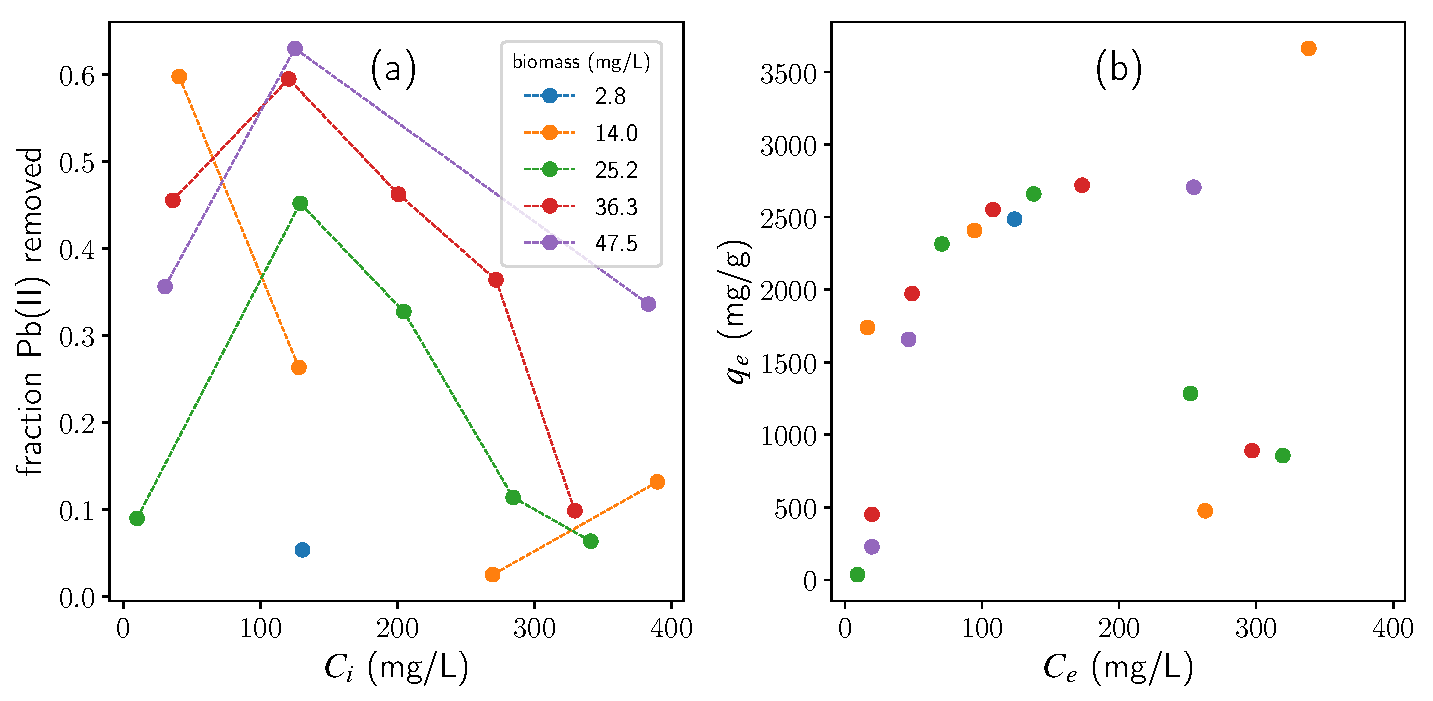
\includegraphics[width=1\linewidth]{Experimental/Pics/conc-vs-rem}
	\caption{The effects of biomass concentration and initial Pb(II) concentration on Pb(II) removal (a) and adsorption capacity (b). The legend shows dry biomass concentration and is shared between both plots.}
	\label{fig:conc-vs-rem}
\end{figure}






\section{Titration}

\subsection{Introduction}




\subsection{Materials and methods}

Acid-base titrations of prepared cultures were performed using an autotitrator (Metrohm 848 Titrino Plus). 

Standard solutions of \SI{0.1}{M} \ce{HNO3} and  \SI{0.1}{M} NaOH were used.

Cells prepared 
dynamic equivalence point titration with autotitrator (Metrohm 848 Titrino Plus).   stability of 50.0 mV/min

100 mL samples purged for 5 min with N2 and maintained throughout experiment.
temp control at 37 +- 1 Celsius
0.1 M NaOH and HNO3
acid added until a pH of 4 reached, increased with NaOH until 10. pH range outside causes cell damage (less than 3) and lysis (greater than 10) \parencite(Kapetas2011).

\subsection{Results and discussion}

\section{Adsorption kinetics}
\section{Adsorption equilibrium}
